\supplementarysection


\begin{longtblr}[
  theme=ntabs,
  caption = {Model information}, % Table caption
  label = {table:model_info} % Label for cross-referencing
  % note{a} = {Continued from previous page}, % Note for continued header
  % note{b} = {Continued on next page}, % Note for continued footer
]{
  colspec = {X[l] X[6,l] X[l] X[l] X[l]}, % Define column specification
  column{1}={colsep=15pt},
  rowhead=1,
  row{odd} = {tablegrey}, % Shading for odd rows
  cells = {font = \fontsize{8pt}{8pt}\selectfont},
  row{1} = {tableheadgrey, font=\fontsize{8pt}{8pt}\selectfont\bfseries} % First row is bold
}

Model & Formula & Family & N & Groups \\

\addlinespace
\SetCell[c=5]{c, white}\textbf{Individual Repertoires} \\

% Individual Repertoires
rep\_m\_1 & repertoire\_size $\sim$ 1 + immigrant + s(sampling\_effort) + year + (1 | father) & cratio & 301 & 242 \\
rep\_m\_1.1 & repertoire\_size $\sim$ 1 + dispersal\_distance + s(sampling\_effort) + year + (1 | father) & cratio & 133 & 105 \\
rep\_m\_1.2 & repertoire\_size $\sim$ 1 + age + s(sampling\_effort) + year + (1 | father) & cratio & 256 & 205 \\
repnov\_m\_1 & average\_frequency $\sim$ 1 + immigrant + s(sampling\_effort) + year + (1 | father) & lognormal & 300 & 242 \\
repnov\_m\_1.1 & average\_frequency $\sim$ 1 + dispersal\_distance + s(sampling\_effort) + year + (1 | father) & lognormal & 133 & 105 \\
repnov\_m\_1.2 & average\_frequency $\sim$ 1 + age + s(sampling\_effort) + year + (1 | father) & lognormal & 256 & 205 \\

% Cultural Similarity
\SetCell[c=5]{c, white}\textbf{Cultural Similarity} \\
disp\_m\_1 & mean\_dist1 $\sim$ 0 + natal\_distance + nest\_distance + year\_born\_diff + year + (1 | mm(father, father2)) & Gaussian & 8745 & 105 \\
imm\_m\_1 & mean\_dist1 $\sim$ 0 + resident\_status + year\_born\_diff + nest\_distance + year + (1 | mm(father, father2)) & Gaussian & 11029 & 205 \\
age\_m\_1 & mean\_dist1 $\sim$ 0 + natal\_distance + nest\_distance + year\_born\_diff + year + (1 | mm(father, father2)) & Gaussian & 8745 & 105 \\

% Cultural Novelty and Diversity
\SetCell[c=5]{c, white}\textbf{Cultural Novelty and Diversity} \\
nov\_m\_1 & uniqueness $\sim$ 0 + prop\_immigrant + mean\_dispersal\_distance + prop\_same\_birds + mean\_age + s(n\_current\_songs) + year + gp(x, y, by = year) & lognormal & 791 & GP \\
div\_m\_1 & diversity $\sim$ 0 + prop\_immigrant + mean\_dispersal\_distance + prop\_same\_birds + mean\_age + s(n\_current\_songs) + year + gp(x, y, by = year) & lognormal & 791 & GP \\
nov\_m\_2 & uniqueness $\sim$ 0 + diversity + s(n\_current\_songs) + year + gp(x, y, by = year) & lognormal & 791 & GP \\
nov\_m\_2.1 & uniqueness $\sim$ 0 + diversity + year + gp(x, y, by = year) & lognormal & 791 & GP \\
div\_m\_2 & n\_unique\_current\_songs $\sim$ 0 + prop\_immigrant + mean\_dispersal\_distance + prop\_same\_birds + mean\_age + s(recorded) + year + gp(x, y, by = year) & Gaussian & 791 & GP \\
div\_m\_2.1 & n\_unique\_current\_songs $\sim$ 0 + prop\_immigrant + mean\_dispersal\_distance + prop\_same\_birds + mean\_age + s(n\_current\_songs) + year + gp(x, y, by = year) & Gaussian & 791 & GP \\

% Cultural Turnover
\SetCell[c=5]{c, white}\textbf{Cultural Turnover} \\
turn\_m\_1 & prop\_shared $\sim$ 0 + prop\_same\_birds + year + gp(x, y, by = year, k = 25, c = 5/4) & hurdle lognormal & 544 & GP \\
turn\_m\_2 & prop\_shared $\sim$ 0 + prop\_immigrant + mean\_dispersal\_distance + mean\_age + prop\_same\_birds + year + gp(x, y, by = year, k = 25, c = 5/4) & hurdle lognormal & 544 & GP \\
\end{longtblr}
\begin{longtblr}[
    theme=ntabs,
    caption = {Model variable key}, % Table caption
    label = {table:variable_key} % Label for cross-referencing
  ]{
    colspec = {X[l] X[6,l]}, % Define column specification
    column{1}={colsep=15pt},
    rowhead=1,
    row{odd} = {tablegrey}, % Shading for odd rows
    cells = {font = \fontsize{8pt}{8pt}\selectfont},
    row{1} = {tableheadgrey, font=\fontsize{8pt}{8pt}\selectfont\bfseries} % First row is bold
  }
  
  Variable & Description \\
  
  repertoire\_size & Number of distinct song types sung by an individual \\
  immigrant & Immigrant status (hatched in the population / not hatched in the population)  \\
  sampling\_effort & Total number of recordings obtained for this individual \\
  year & Year in which the repertoire was recorded \\
  father & ID of the male; BTO (British Trust for Ornithology) ring number \\
  dispersal\_distance & Postnatal dispersal distance, in metres, from the natal nest box to the breeding nest box \\
  age & The age of the bird. This is exact if the bird was ringed as a pullus in the population, or approximate (based on plumage moult) otherwise \\
  average\_frequency & The mean of the frequency of each song in a bird's repertoire in a given year \\
  mean\_dist1 & Average minimum Euclidean distance between the repertoires of two birds \\
  natal\_distance & Distance in metres at which two birds were born \\
  nest\_distance & Distance in metres at which two birds bred \\
  year\_born\_diff & The absolute difference between the birth years of two birds \\
  mm(...) & Multi-membership grouping term for the similarity network \\
  resident\_status & Origin of a pair of birds: both, one or neither were hatched in the population \\
  prop\_immigrant & Proportion of  the birds in a neighbourhood that were not hatched inside the population \\
  mean\_dispersal\_\allowbreak distance & Mean postnatal dispersal distance, in metres, of the birds in the neighbourhood\\
  prop\_same\_birds &  Proportion of the birds in a neighbourhood that were already there the year before \\
  mean\_age & Mean age of the birds in a neighbourhood \\
  n\_current\_songs & Absolute number of song types in a neighbourhood (not unique song types), which correlates with neighbourhood size but we use to further adjust for the fact that some birds sing more songs \\
  gp(x, y) & 2D Gaussian process to model spatial dependency in the data  \\
  n\_unique\_\allowbreak current\_songs & Number of unique song types in a neighbourhood \\
  uniqueness &  The uniqueness of a bird's repertoire, quantified as 1 minus the logarithm of the mean frequency of the songs in its repertoire for a given year  \\
  recorded & Number of birds recorded singing in a neighbourhood, which is linearly correlated with neighbourhood size \\
  prop\_shared & Proportion of the song types in a neighbourhood that were already present. Reported as 1- prop\_shared: 'song turnover'\\
  \end{longtblr}
\begin{longtblr}[
  theme=ntabs,
  caption = {Model estimates}, % Table caption
  label = {table:model_estimates}, % Label for cross-referencing
  note{a} = {Estimates are Medians and 95\% Credible Intervals}, % Note for continued header
]{
  colspec = {X[l] X[3,l] X[3,l] X[1.5,l] X[1.5,l]}, % Define column specification
  column{1}={colsep=15pt},
  rowhead=1,
  % rowsep=0pt,
  row{odd} = {tablegrey}, % Shading for odd rows
  cells = {font = \fontsize{8pt}{8pt}\selectfont},
  row{1} = {tableheadgrey, font=\fontsize{8pt}{8pt}\selectfont\bfseries} % First row is bold
}

Model & Hypothesis & Estimate\TblrNote{a} & Evid. Ratio & Post. Prob \\

\addlinespace
\SetCell[c=5]{c, white}\textbf{Individual Repertoires} \\

% Individual Repertoires
rep\_m\_1 & immigrant $>$ 0 & 0.239 [-0.098, 0.593] & 6.963 & 0.874 \\
rep\_m\_1.1 & dispersal distance $<$ 0 & -0.201 [-0.443, 0.045] & 10.111 & 0.910 \\
rep\_m\_1.2 & age $>$ 0 & 0.064 [-0.108, 0.241] & 2.701 & 0.730 \\
repnov\_m\_1 & non-immigrant $<$ 0 & -0.049 [-0.2, 0.1] & 2.401 & 0.706 \\
repnov\_m\_1.1 & dispersal distance $>$ 0 & 0.203 [0.088, 0.316] & 741.857 & 0.999 \\
repnov\_m\_1.2 & age $>$ 0 & -0.017 [-0.093, 0.058] & 0.540 & 0.351 \\

% Cultural Similarity
\SetCell[c=5]{c, white}\textbf{Cultural Similarity} \\
disp\_m\_1 & natal distance $>$ 0 & 0.001 [0, 0.002] & 22.529 & 0.958 \\
disp\_m\_1 & nest distance $>$ 0 & -0.005 [-0.006, -0.004] & Inf & 1 \\
imm\_m\_1 & both resident-both immigrant $<$ 0 & 0.002 [-0.005, 0.01] & 0.438 & 0.304 \\
imm\_m\_1 & both resident-one immigrant $<$ 0 & 0.002 [-0.002, 0.006] & 0.331 & 0.248 \\
age\_m\_1 & age difference 0-1 $>$ 0 & 0.002 [0, 0.003] & 12.289 & 0.925 \\
age\_m\_1 & age difference 0-2 $>$ 0 & 0.004 [0.002, 0.006] & Inf & 1 \\
age\_m\_1 & age difference 0-3 $>$ 0 & 0.006 [0.003, 0.008] & 1999 & 1 \\
age\_m\_1 & age difference 0-4+ $>$ 0 & 0.01 [0.006, 0.013] & Inf & 1 \\

% Cultural Novelty and Diversity
\SetCell[c=5]{c, white}\textbf{Cultural Novelty and Diversity} \\
nov\_m\_1 & mean dispersal distance $<$ 0 & -0.018 [-0.023, -0.012] & Inf & 1 \\
nov\_m\_1 & proportion immigrant $<$ 0 & 0.001 [-0.005, 0.006] & 0.752 & 0.429 \\
nov\_m\_1 & mean age $<$ 0 & 0.012 [0.005, 0.019] & 399 & 0.998 \\
nov\_m\_1 & individual turnover $<$ 0 & 0.001 [-0.005, 0.008] & 1.733 & 0.634 \\
div\_m\_1 & mean dispersal distance $<$ 0 & -0.005 [-0.01, 0] & 26.65 & 0.964 \\
div\_m\_1 & proportion immigrant $<$ 0 & 0.002 [-0.004, 0.007] & 0.442 & 0.306 \\
div\_m\_1 & mean age $<$ 0 & 0.021 [0.014, 0.027] & Inf & 1 \\
div\_m\_1 & individual turnover $<$ 0 & -0.002 [-0.008, 0.005] & 0.446 & 0.309 \\
nov\_m\_2 & diversity $>$ 0 & 0.713 [0.629, 0.795] & Inf & 1 \\
nov\_m\_2.1 & diversity $>$ 0 & -0.099 [-0.216, 0.018] & 0.086 & 0.080 \\
div\_m\_2 & mean dispersal distance $<$ 0 & -0.658 [-0.999, -0.315] & 570.429 & 0.998 \\
div\_m\_2 & proportion immigrant $<$ 0 & 0.469 [0.1, 0.837] & 62.492 & 0.984 \\
div\_m\_2 & mean age $<$ 0 & 1.045 [0.576, 1.495] & Inf & 1 \\
div\_m\_2 & individual turnover $<$ 0 & 0.204 [-0.291, 0.683] & 3.077 & 0.755 \\
div\_m\_2.1 & mean dispersal distance $<$ 0 & 0.019 [-0.213, 0.249] & 0.824 & 0.452 \\
div\_m\_2.1 & proportion immigrant $<$ 0 & 0.072 [-0.168, 0.312] & 2.259 & 0.693 \\
div\_m\_2.1 & mean age $<$ 0 & 0.928 [0.599, 1.245] & Inf & 1 \\
div\_m\_2.1 & individual turnover $<$ 0 & -0.031 [-0.349, 0.279] & 0.726 & 0.421 \\

% Cultural Turnover
\SetCell[c=5]{c, white}\textbf{Cultural Turnover} \\
turn\_m\_1 & individual turnover $>$ 0 & 0.072 [0.054, 0.09] & Inf & 1 \\
turn\_m\_2 & mean dispersal distance $<$ 0 & -0.022 [-0.039, -0.006] & 79 & 0.988 \\
turn\_m\_2 & proportion immigrant $<$ 0 & -0.051 [-0.065, -0.037] & Inf & 1 \\
turn\_m\_2 & mean age $<$ 0 & -0.044 [-0.063, -0.026] & 3999 & 1 \\
turn\_m\_2 & individual turnover $<$ 0 & 0.047 [0.028, 0.066] & Inf & 1 \\
\end{longtblr}



\begin{figure}[tbp]
    \centering
    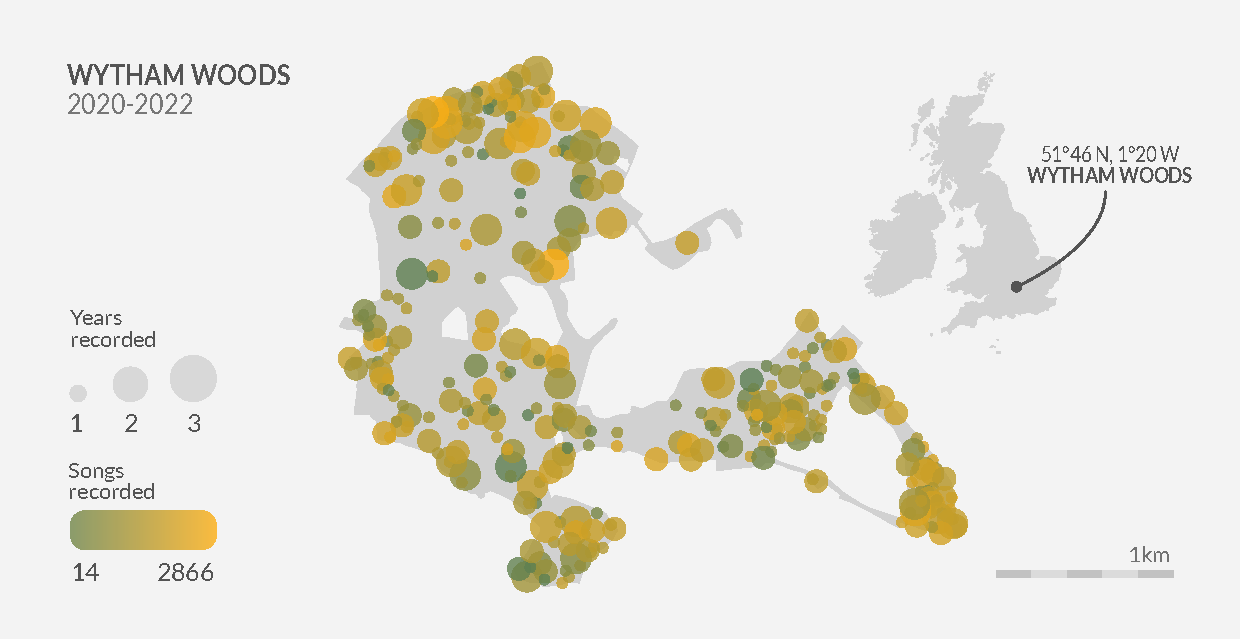
\includegraphics[width=\linewidth]{figures/chapter_4/supp_study_site.pdf}
    \mycaption{Map of the study site and sampling locations}{
        This study was conducted in Wytham Woods, a 385-hectare semi-natural woodland surrounded by farmland. Data was collected during the breeding seasons of 2020, 2021, and 2022 by regularly checking 1018 nest boxes, documenting information such as breeding pair identities, clutch initiation and hatching dates, clutch size, and fledgling details according to standardized protocols, and recording the songs of the birds in the population using 60 AudioMoth acoustic loggers. The map shows the location of the nest boxes where we recorded song repertoires.
    }
    \label{fig:supp_study_site}
\end{figure}



\begin{figure}[tbp]
    \centering
    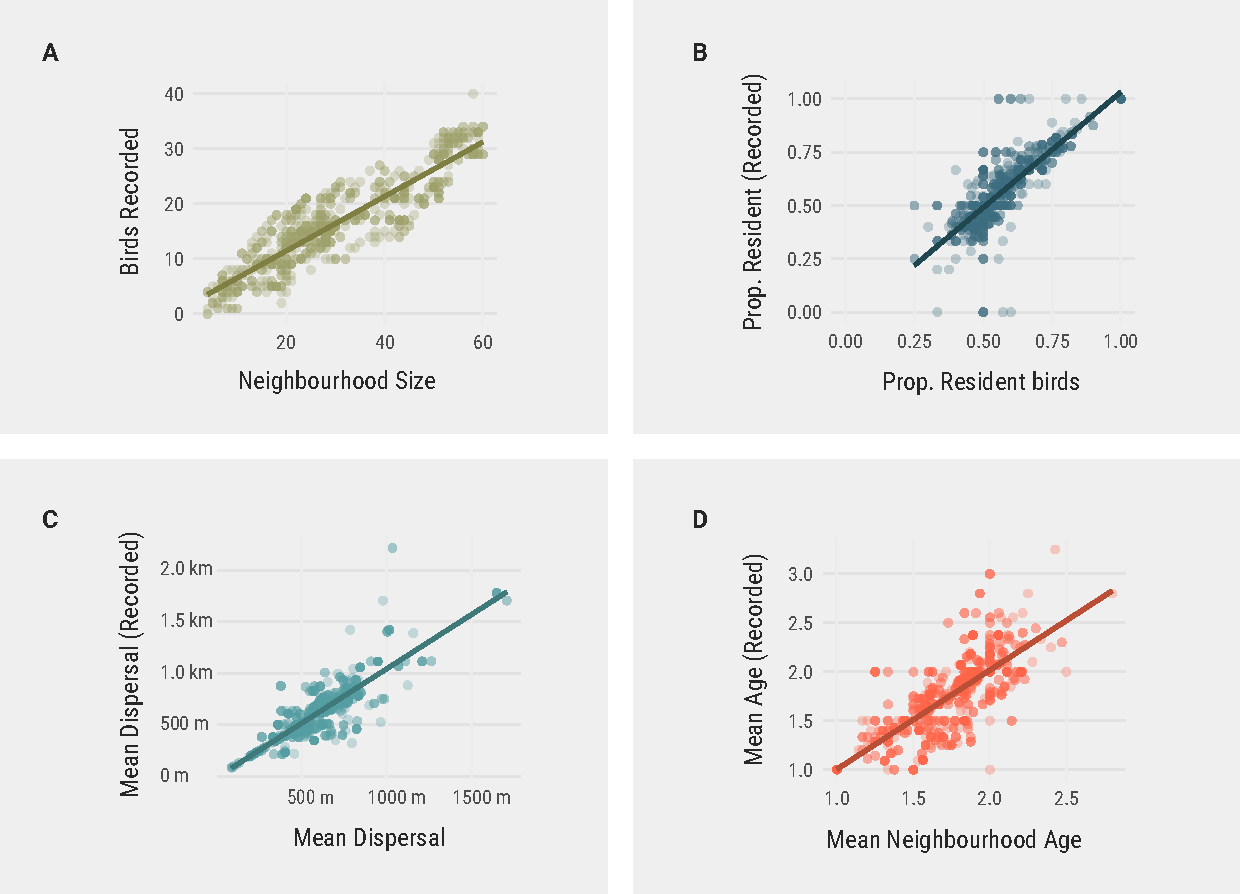
\includegraphics[width=\linewidth]{figures/chapter_4/supp_neighbourhood_sampling.pdf}
    \mycaption{Demographic characteristics of recorded birds compared to those of all birds in the neighbourhood}{
        Comparison between the actual neighbourhood properties and neighbourhood properties estimated from birds for which we have song recordings.
    (A) Neighbourhood size (number of individuals) and number of individuals for which we have song recordings in that same neighbourhood.
    (B) Proportion of resident birds calculated from monitoring data and only from those birds with song recordings. Residents are birds that were ringed as nestlings in the population.
    (C) Mean dispersal distance of the birds in a neighbourhood calculated from monitoring data and only from birds with song recordings.
    (D) Mean age of birds in a neighbourhood calculated from monitoring data and only from birds with song recordings.
    }
    \label{fig:supp_neighbourhood_sampling}
\end{figure}


\begin{figure}[tbp]
    \centering
    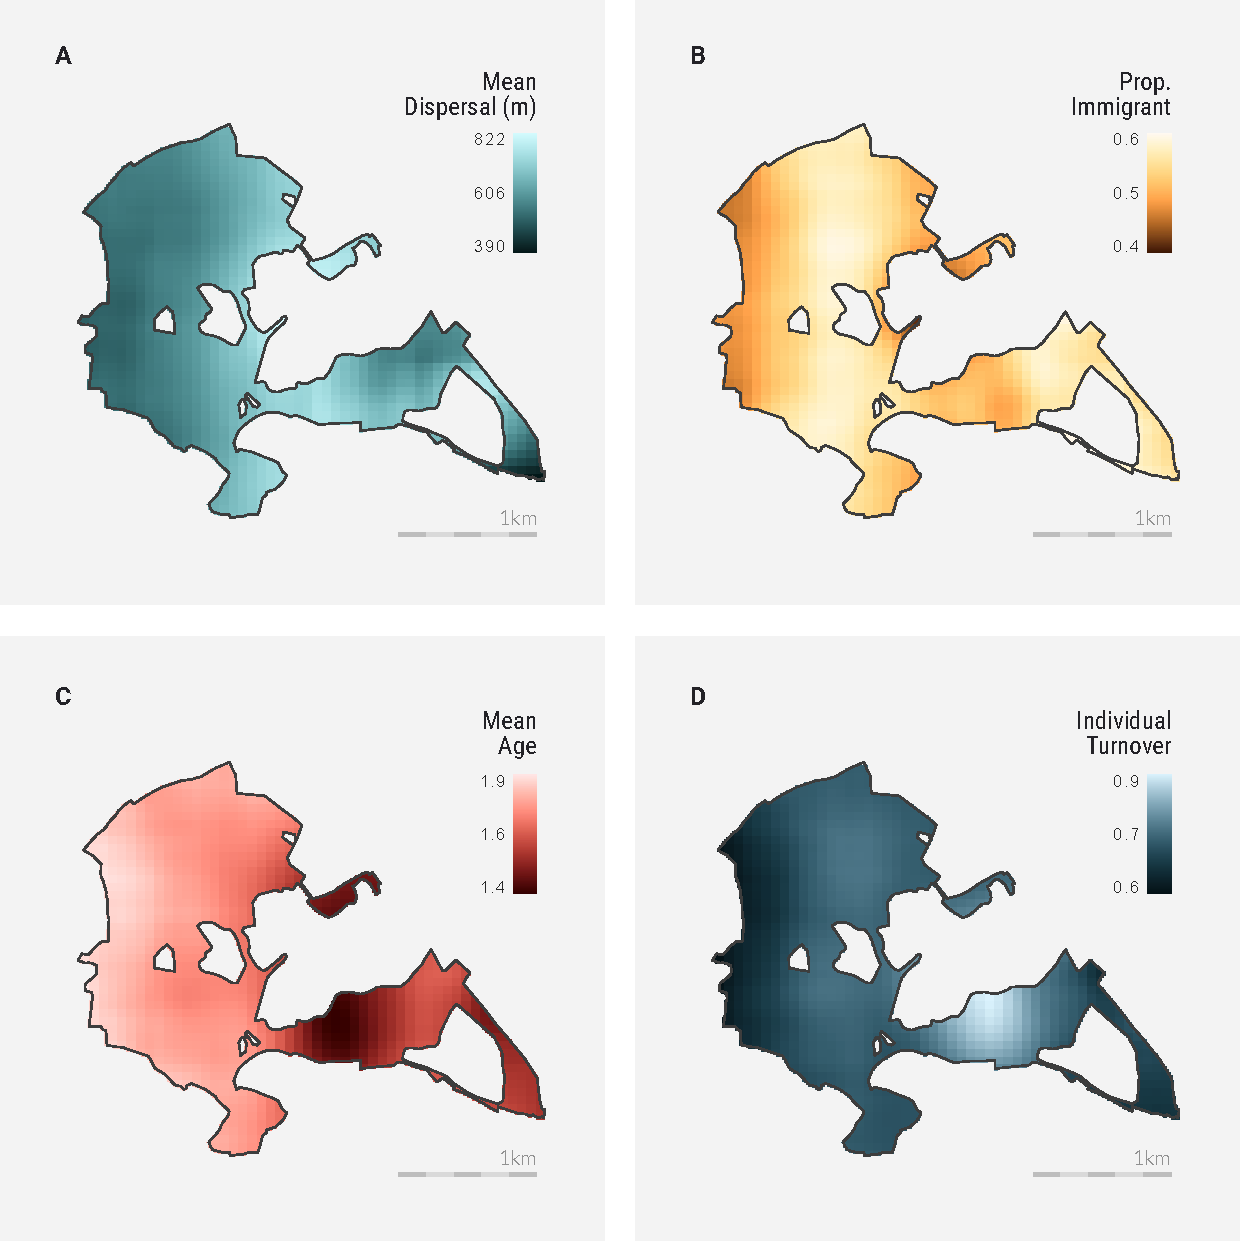
\includegraphics[width=\linewidth]{figures/chapter_4/supp_demo_variables.pdf}
    \mycaption{Spatial distribution of the neighbourhood-level predictor variables in the study}{
    (A) Mean natal dispersal distance, or the mean distance between the natal nest box and the breeding site for all birds in the neighbourhood.
    (B) Proportion of immigrant birds in the neighbourhood.
    (C) Mean age of birds in the neighbourhood.
    (D) Individual turnover, or the proportion of birds that were not already in a neighbourhood in the preceding year.
    }
    \label{fig:supp_demo_variables}
\end{figure}

\begin{figure}[tbp]
    \centering
    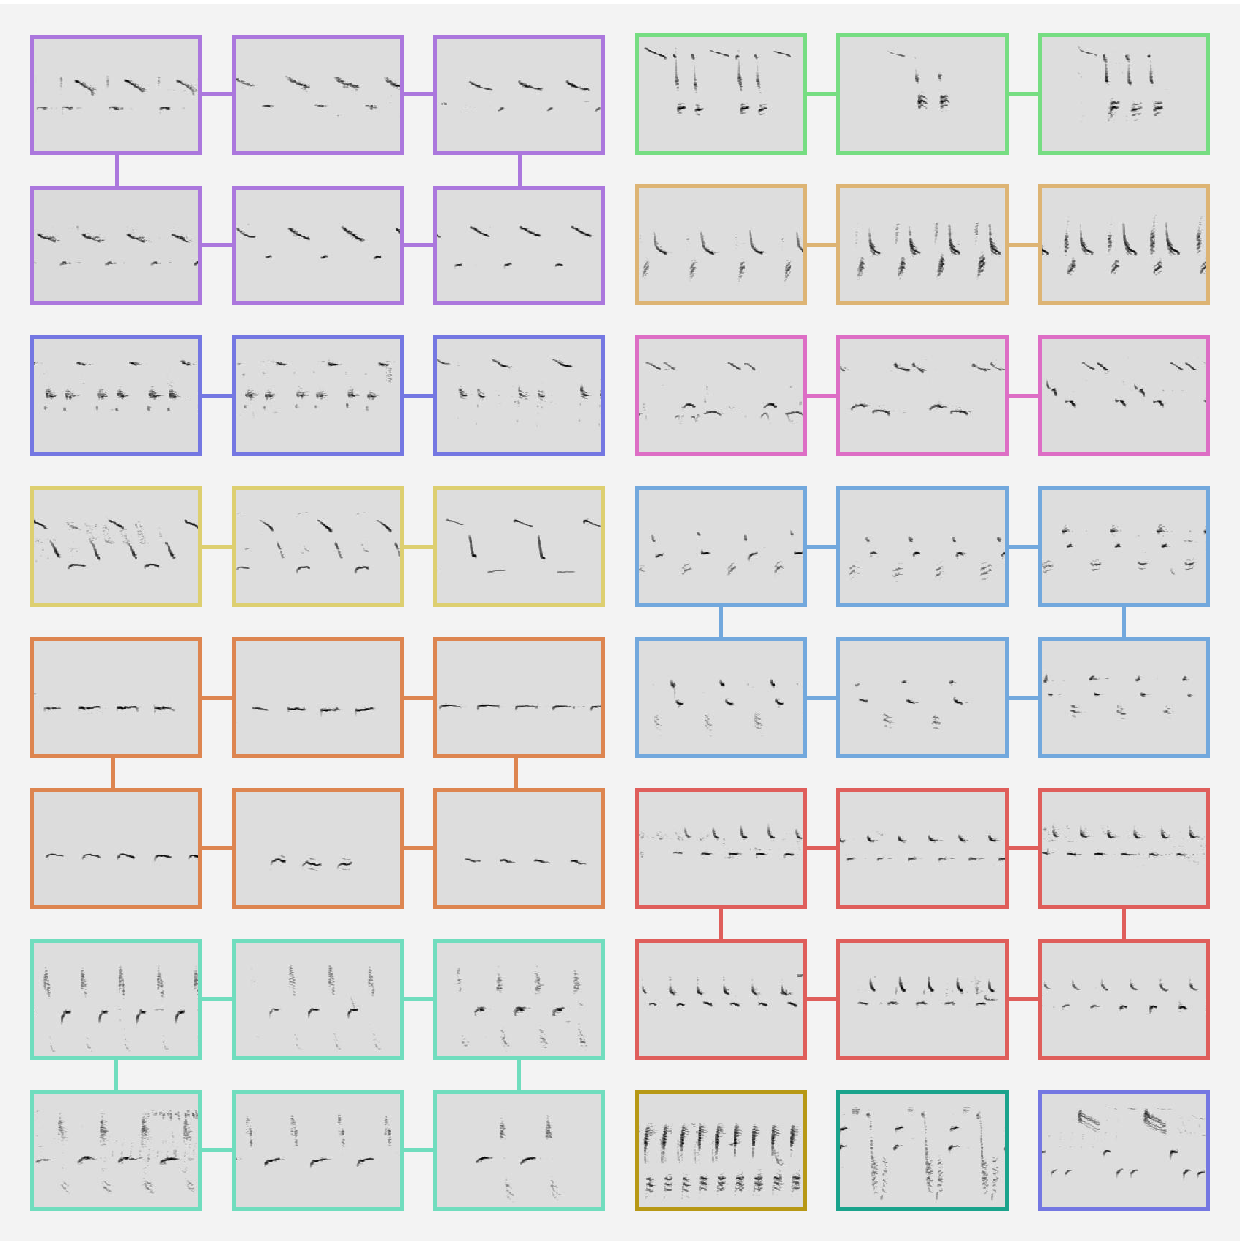
\includegraphics[width=\linewidth]{figures/chapter_4/supp_song_typle_clusters.pdf}
    \mycaption{Examples of song type clusters in the study population}
    {
Colours and connected lines represent the same song type cluster sung by different birds. Some song types are sung by many birds, while others are unique to a single bird. The clustering process is based on song similarity derived from a deep metric learning model and a manual categorization process following McGregor and Krebs \autocite{mcgregor1982b}.
    }
    \label{fig:supp_song_typle_clusters}
\end{figure}


\begin{figure}[tbp]
    \centering
    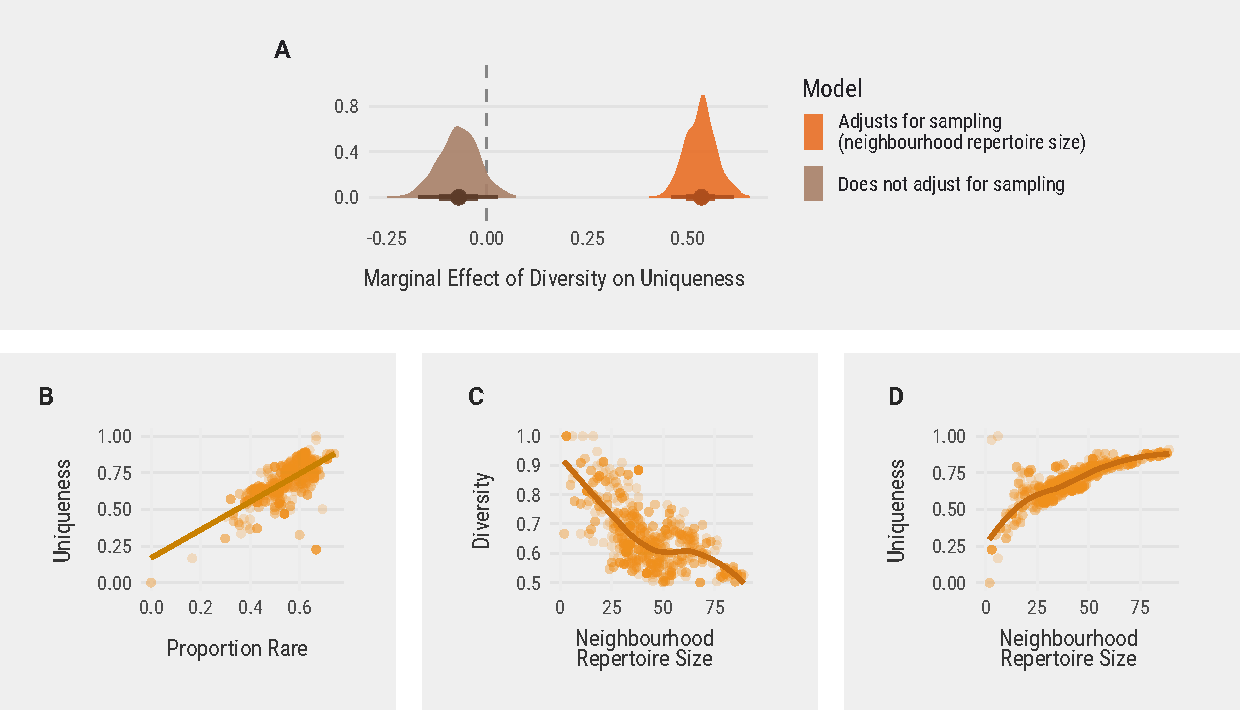
\includegraphics[width=\linewidth]{figures/chapter_4/supp_song_sampling.pdf}
    \mycaption{Estimates of cultural outcomes depend on the size of the neighbourhood repertoire}
    {
        (A) Marginal effect of diversity---which describes the proportion of unique songs in a neighbourhood---on uniqueness, that is, how uncommon, on average, the songs of the birds in a neighbourhood are. These two ways of characterizing cultural diversity are anti-correlated in our study site due to the effect of sampling: more frequent songs are sampled more readily, causing larger sample sizes (neighbourhoods with more birds and therefore songs) to yield lower average estimates of diversity (C) and higher average estimates of uniqueness (D), in a nonlinear manner. Once this is adjusted for, which we do by including GAM terms capturing neighbourhood song density or number of birds, diversity and uniqueness are positively correlated, as expected. (B) Our measure of cultural uniqueness (y-axis) has the advantages of being continuous and not using an arbitrary cut-off, but is nonetheless correlated with definitions traditionally used in the literature, such as 'songs shared by fewer than 4 birds” \autocite{mcgregor1982b}, here on the x-axis.}
    \label{fig:supp_song_sampling}
\end{figure}

\begin{figure}[tbp]
    \centering
    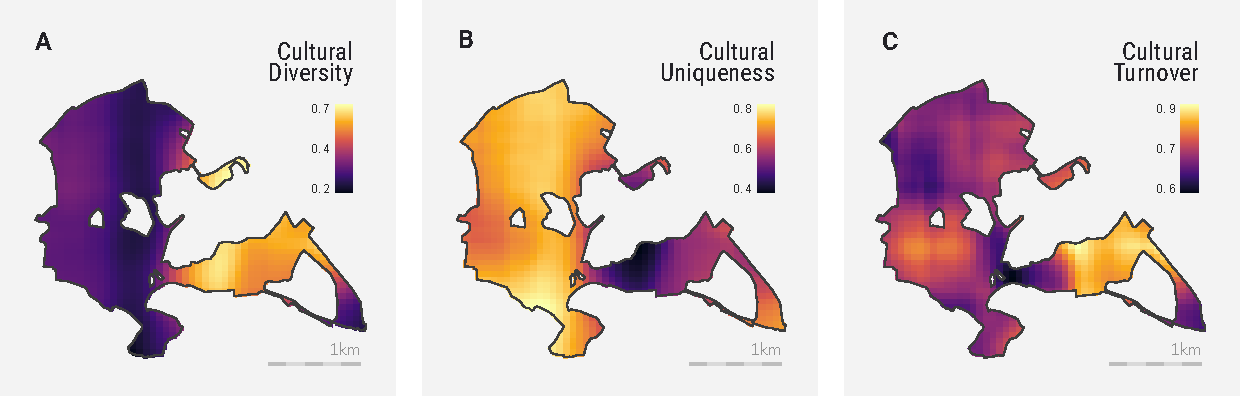
\includegraphics[width=\linewidth]{figures/chapter_4/supp_cultural_variables.pdf}
    \mycaption{Spatial distribution of the neighbourhood-level cultural variables in the study}
    {
        (A) Relative diversity, or the proportion of unique songs in a neighbourhood.
        (B) Uniqueness, or how uncommon, on average, the songs of the birds in a neighbourhood are.
        (C) Rate of song cultural turnover, or the proportion of unique song types in a given year that were not already present in the same neighbourhood the preceding year.
        As described in \autoref{fig:supp_song_sampling}, (A) and (B) are anti-correlated due to the effect of sampling, but once this is adjusted for, neighbourhoods with more cultural diversity also tend to have more unique songs, as expected.
        }
    \label{fig:supp_cultural_variables}
\end{figure}

\begin{figure}[tbp]
    \centering
    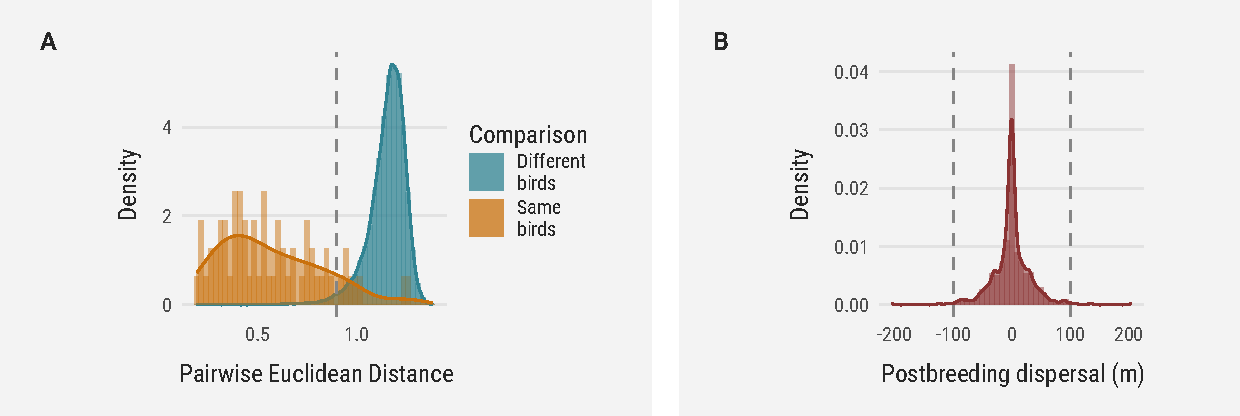
\includegraphics[width=\linewidth]{figures/chapter_4/supp_acoustic_distance_threshold.pdf}
    \mycaption{Thresholds used during the process of reidentifying individual birds based on their songs}{
        (A) Shows the distribution of the acoustic distances between the same song type sung by the same known bird in different years, in orange, and the minimum pairwise distance between different birds and years. The x-intercept of the vertical line = 0.9. (B) Shows the distribution of the change in distance from the natal nest box to the breeding site in different years for birds that bred more than once. Adult birds have high nest site fidelity, which we used as a further constraint when reidentifying them from their songs.}
    \label{fig:supp_acoustic_distance_threshold}
\end{figure}


\begin{figure}[tbp]
    \centering
    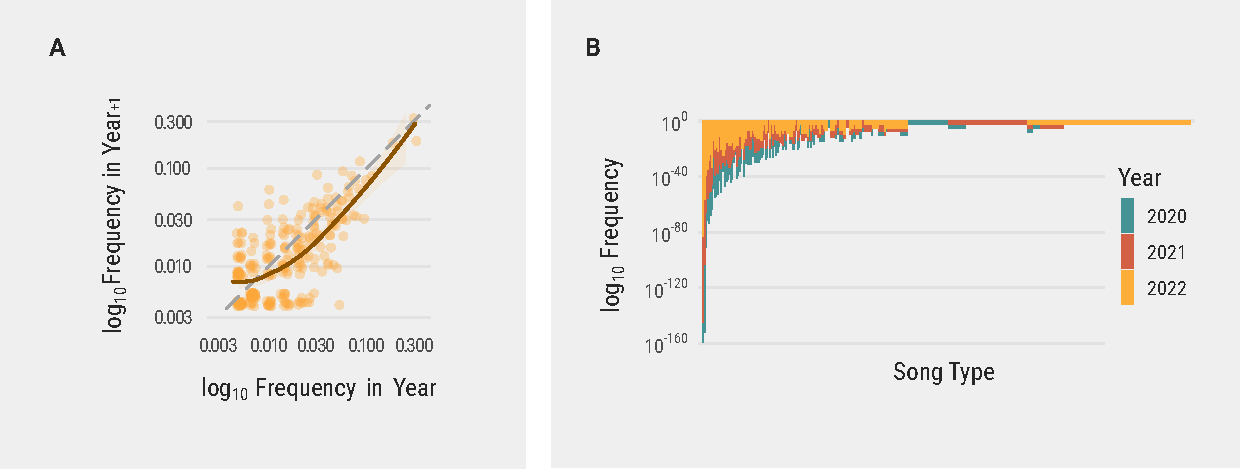
\includegraphics[width=\linewidth]{figures/chapter_4/supp_song_frequencies.pdf}
    \mycaption{
        Song frequencies and their relationship with abundance in the following year}{
        (A) The abundance of a song type in a given year predicts its abundance in the following year, with higher variance around rare songs. (B) Histogram showing the frequency of individual song types in the study.
    }
    \label{fig:supp_song_frequencies}
\end{figure}

\begin{figure}[tbp]
    \centering
    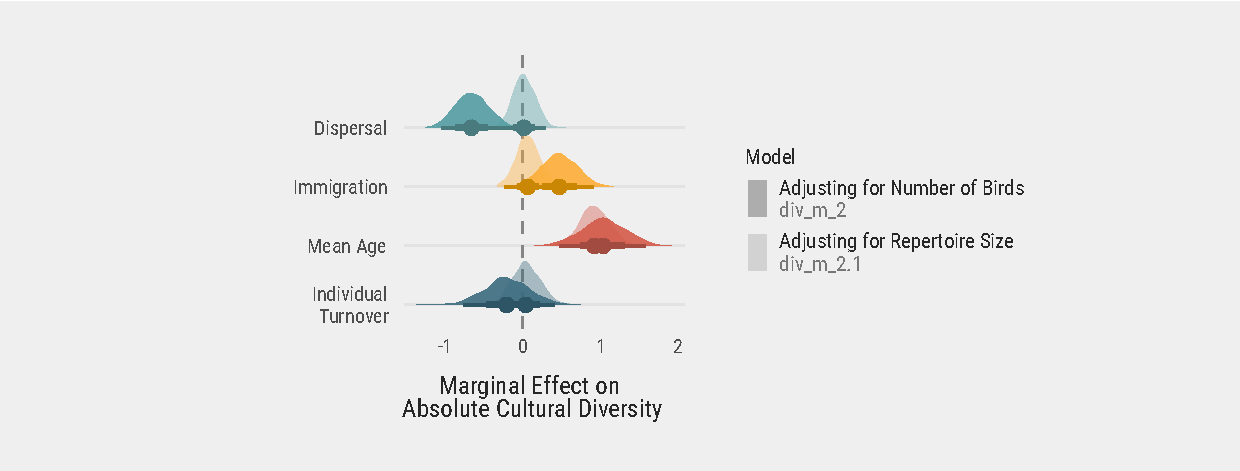
\includegraphics[width=\linewidth]{figures/chapter_4/supp_absolute_cultural_diversity.pdf}
    \mycaption{Effect of demographic variation on absolute cultural diversity within neighbourhoods}{
        To explore how the number of individuals and their repertoire sizes within a neighbourhood affect the absolute number of different song types (as opposed to the relative diversity reported in \autoref{c4_fig:diversity}), we fit two models: one adjusting for the nonlinear effect of the number of individuals (higher opacity fill, corresponding to model \textit{div\_m\_2}), and a second adjusting for the nonlinear effect of the number of song types, including repeated variants (lower opacity fill, \textit{div\_m\_2.1}). See \autoref{table:model_info} for full model specifications.
    }
    \label{fig:supp_absolute_cultural_diversity}
\end{figure}

\begin{figure}[tbp]
    \centering
    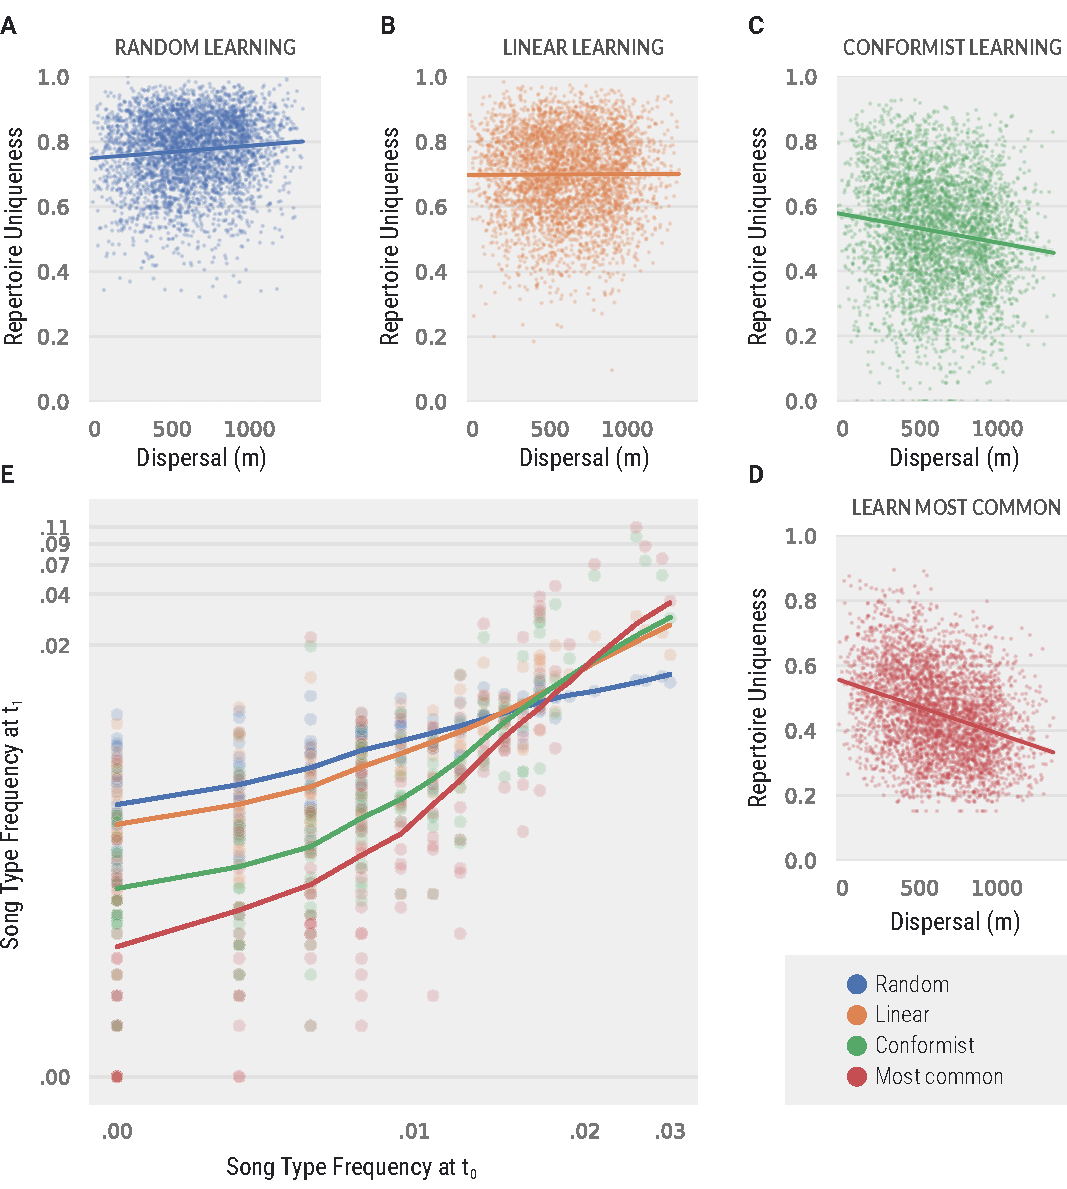
\includegraphics[width=\linewidth]{figures/chapter_4/supp_dispersal_simulation.pdf}
    \mycaption{Simulation of the effect of natal dispersal on repertoire uniqueness}
    {
        We simulate the relationship between pre-breeding bird movement and the uniqueness of songs in their repertoires  (relative to the population). We initialize 200 birds in a 1500 x 1500 square, each capable of singing 4 songs selected from
        a pool of 200 song types. Birds do not initially move. New birds are born and move based on a log-normal distribution parametrized to represent realistic dispersal behaviour in our population. Each bird can learn the songs it hears within a 200 m radius as it moves. At the end of their movement, a bird's crystallized repertoire is determined by its learning mechanism: (A) random learning of songs, (B) linearly frequency-dependent learning, (C) positively frequency-dependent learning, or (D) learn the most popular songs (strong conformism). The simulation is repeated $n$ times per learning strategy, and we record the average uniqueness of songs in each bird's repertoire, which is a transformation of the average frequency of the bird's songs, as well as the distance that each bird has moved. The results show that the relationship between dispersal and repertoire uniqueness depends on the learning mechanism, and that the effect of dispersal detected in our study might be expected to arise if being exposed to a larger number of songs influences learning in a nonlinear frequency-dependent manner.
    }
    \label{fig:supp_dispersal_simulation}
\end{figure}


\begin{figure}[tbp]
    \centering
    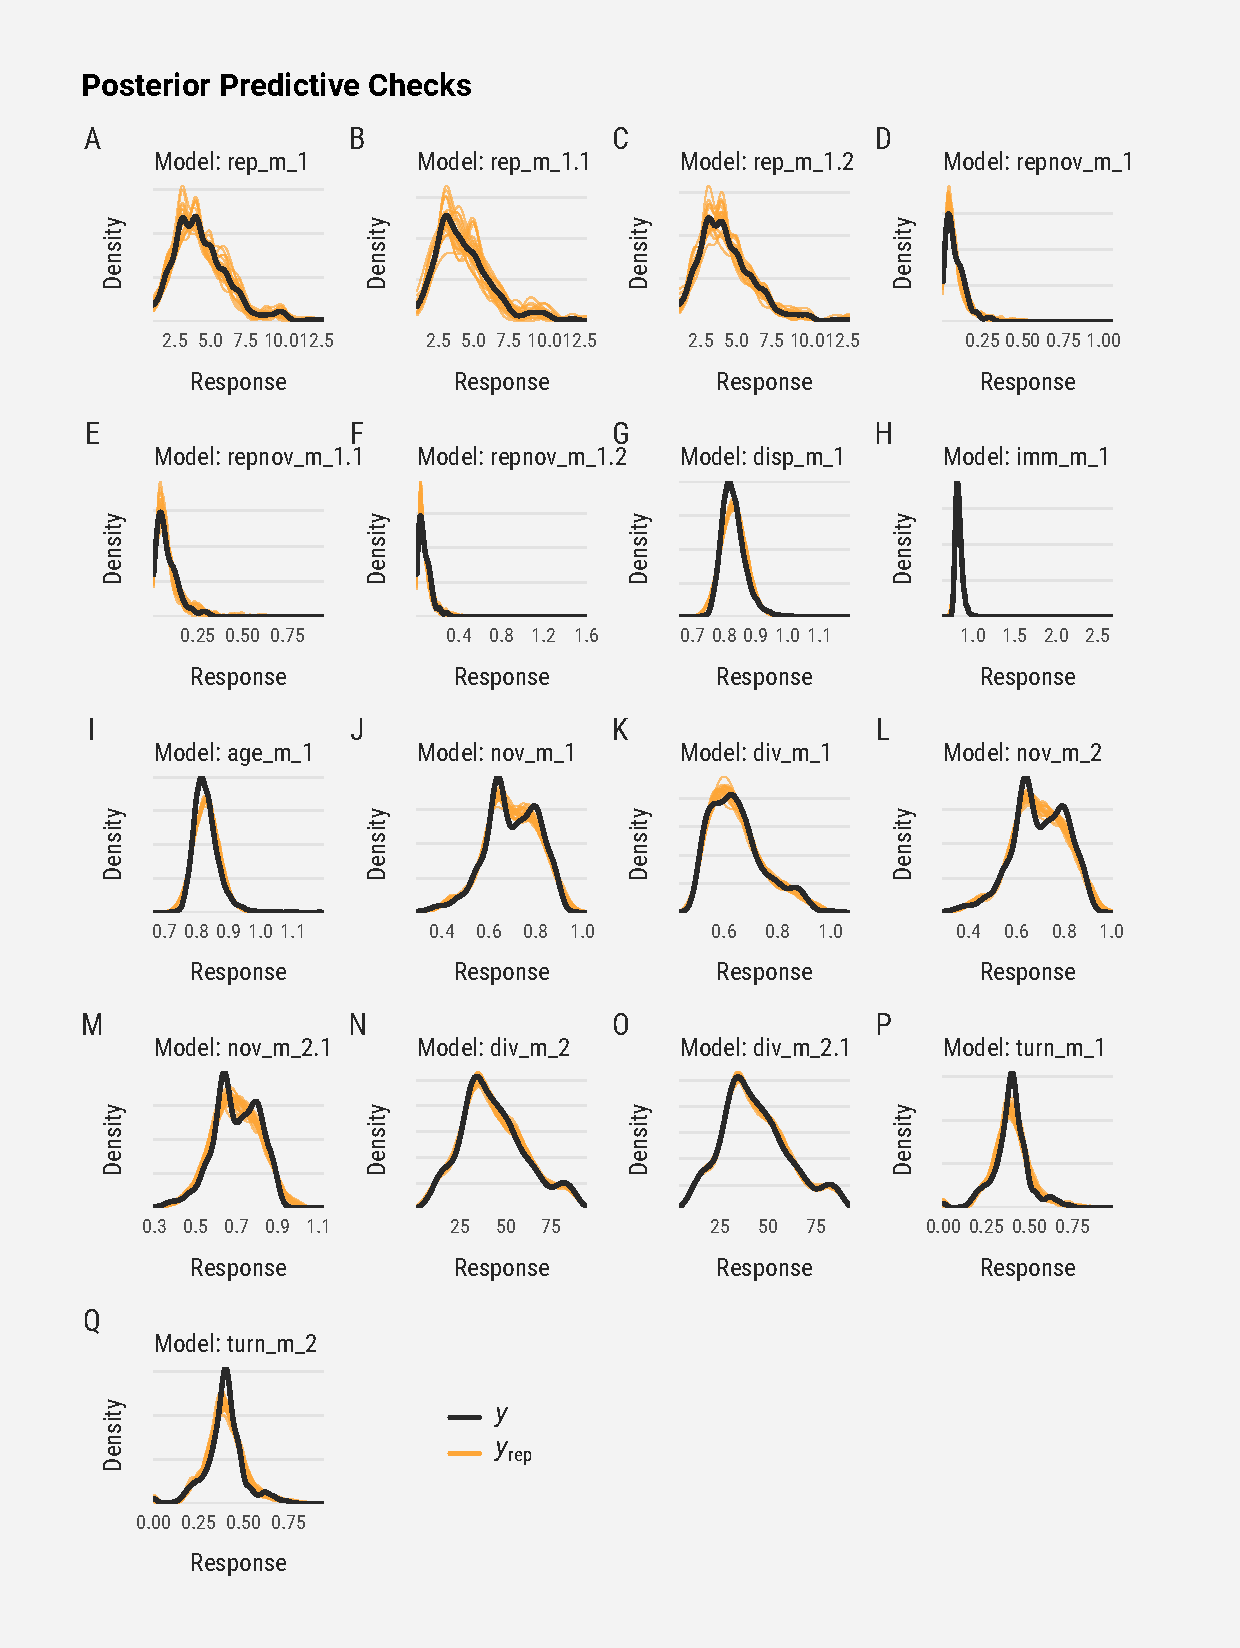
\includegraphics[width=\linewidth]{figures/chapter_4/supp_pp_checks.pdf}
    \mycaption{
        Posterior predictive checks for the main models in the study}{Comparing simulations from the posterior predictive distribution $y^{rep}$ (thin orange lines) with the outcome $y$ (black lines) using Kernel density estimates. The posterior predictive distribution is a distribution of possible outcomes of the model given the data and the model parameters, here used to check the fit of the model to the data.
    }
    \label{fig:supp_pp_checks}
\end{figure}
